% !TeX document-id = {d8b4925c-2057-42a4-b894-2f1a3f1b6345}
%!TeX TXS-program:compile = txs:///xelatex/[--shell-escape]
\documentclass[aspectratio=169, mathserif]{beamer}	% TPU recommends 16:9 ratio, 4:3 may require some work with inner theme .sty file

% Style options:
% light --- light theme (default)
% dark --- dark theme
% enlogo --- english TPU logo {default}
% rulogo --- russian TPU logo

\usetheme[light, rulogo]{tpu}		% dark theme used as an example of optional argument

\usepackage[english, russian]{babel}		%uncomment this to work in russian
\usepackage[utf8]{inputenc}
\usepackage[T2A]{fontenc}

\usepackage{fontspec}

\setromanfont{Brygada1918}[
Path=./fonts/BrygadaFontFiles/,
Extension = .ttf,
UprightFont=*-Regular,
BoldFont=*-Bold,
ItalicFont=*-Italic,
BoldItalicFont=*-BoldItalic
]

\setsansfont{ALSSirius}[
Path=./fonts/ALSSiriusFiles/,
Extension = .otf,
UprightFont=*-Regular,
BoldFont=*-Bold,
%ItalicFont=*-Italic,
%BoldItalicFont=*-BoldItalic
]

\setmonofont{Consolas}[
Path=./fonts/ConsolasFontFiles/,
%Scale=0.85,
Extension = .ttf,
UprightFont=*-Regular,
BoldFont=*-Bold,
ItalicFont=*-Italic,
BoldItalicFont=*-BoldItalic
]

\usepackage[cache=false]{minted}
\usepackage{xcolor} % to access the named colour LightGray
\definecolor{LightGray}{gray}{0.9}
\definecolor{onedarkBckGr}{RGB}{40, 44, 52}

\usemintedstyle[python]{default}
\setminted[python]{
	fontsize=\scriptsize,
	escapeinside=||,
	mathescape=true,
	numbersep=5pt,
	gobble=2,
	linenos=true,
	frame=leftline,
	framesep=1mm,
	python3=true,
}

\usemintedstyle[pycon]{default}
\setminted[pycon]{
	fontsize=\scriptsize,
	escapeinside=||,
	mathescape=true,
	numbersep=5pt,
	gobble=2,
	frame=none,
	framesep=1mm,
	python3=true,
	linenos=false,
}

\usemintedstyle[numpy]{default}
\setminted[numpy]{
	fontsize=\scriptsize,
	escapeinside=||,
	mathescape=true,
	numbersep=5pt,
	gobble=2,
	linenos=false,
	frame=lines,
	framesep=1mm,
	python3=true,
	bgcolor=backcolour,
	linenos=false,
}

\usepackage{booktabs}	% good looking tables
\usepackage{multicol}	% text in multiple columns, useful for side-by-side text and pictures
\usepackage{hyperref}
%\usepackage{minted}
\usepackage{xcolor}
\definecolor{maroon}{cmyk}{0, 0.87, 0.68, 0.32}
\definecolor{halfgray}{gray}{0.55}
\definecolor{ipython_frame}{RGB}{207, 207, 207}
\definecolor{ipython_bg}{RGB}{247, 247, 247}
\definecolor{ipython_red}{RGB}{186, 33, 33}
\definecolor{ipython_green}{RGB}{0, 128, 0}
\definecolor{ipython_cyan}{RGB}{64, 128, 128}
\definecolor{ipython_purple}{RGB}{170, 34, 255}
\definecolor{linkcolor}{HTML}{0000FF} % цвет гиперссылок
\definecolor{urlcolor}{HTML}{800080} % цвет ссылок
\definecolor{backcolour}{rgb}{0.95,0.95,0.92}

\usepackage{amsxtra}
\usepackage{longtable}
\usepackage{wrapfig}
\usepackage{ragged2e}
\usepackage[nooneline]{caption}
\DeclareCaptionTextFormat{center}{\centering{#1}}
\DeclareCaptionLabelFormat{figure}{Рисунок~#2}
\captionsetup[table]{justification=raggedleft,
	labelformat=empty,
	labelsep=endash,
	textformat=center,
	position=top,
	skip=5pt
}
\captionsetup[figure]{justification=centering,
	labelsep=endash,
	labelformat=figure,
	font={tiny}
}


\hyphenpenalty=10000	% i don’t think hyphenation in presentations is a good idea, feel free to change however you like


%\includeonlyframes{o}

\title{\Large{Системный анализ процессов переработки нефти и газа}}
\subtitle{\textcolor{tpugreen}{\textbf{Лекция 6}} \\ \textbf{Основы объектно-ориентированного \\ программирования (ООП)}}
\author[]{\textbf{Вячеслав Алексеевич Чузлов}}
\institute{к.т.н., доцент ОХИ ИШПР}
\date{\today}

\begin{document}

% notice usage of \titleframe and several other unconventional functions
% the reason being is custom backgrounds on these slides

\titleframe		% title

\tocframe{}		% this custom frame accepts options for ToC

%\addcontentsline{toc}{section}{\textbf{I Численные методы решения систем \\ линейных уравнений}}



\section{Объектно-ориентированное \\ программирование на языке Python}
\sectionframe

\begin{frame}[fragile]{Объектно-ориентированное программирование}
\scriptsize
\begin{itemize}
	\item \textcolor{tpugreen}{\textbf{Классы}} и \textcolor{tpugreen}{\textbf{объекты}}~-- это два основных аспекта объектно-ориентированного программирования. Класс создаёт новый тип, а объекты являются экземплярами класса.
%	\vfill
	\item Объекты могут хранить данные в обычных переменных, которые принадлежат объекту.
%	\vfill
	\item Переменные, принадлежащие объекту или классу, называют \textcolor{extraorange}{\textbf{полями}} или \textcolor{extraorange}{\textbf{свойствами}}.
%	\vfill
	\item Объекты могут также обладать функционалом, т.е. иметь функции, принадлежащие классу. Такие функции принято называть \textcolor{extraorange}{\textbf{методами}} класса.
%	\vfill
	\item Всё вместе (поля и методы) принято называть \textcolor{extraorange}{\textbf{атрибутами}} класса.
\end{itemize}
\vfill
Описание простейшего класса:
\begin{minted}{python}
class Person:
    pass


petr = Person()
ivan = Person()
print(petr)
|\space|
\end{minted}
\begin{minted}{pycon}
<__main__.Person object at 0x0000026354CDBA30>
\end{minted}
\vfill
\end{frame}

\subsection{Конструктор класса}
\begin{frame}[fragile]{Объектно-ориентированное программирование}
\scriptsize
\textcolor{tpugreen}{\textbf{Конструктор класса}}~-- это специальный блок инструкций, вызываемый при создании объекта. В Python это метод \mintinline{python}|__init__()|.
\vfill
\begin{minted}{python}
class Person:
    def __init__(self, name: str, surname: str) -> None:
        self.name = name
        self.surname = surname


person = Person(name='Петр', surname='Петров')
print(f'Привет, {person.name} {person.surname}!')

for person in [Person('Максим', 'Иванов'), Person('Мария', 'Петрова')]:
    print(f'Привет, {person.name} {person.surname}!')
|\space|
\end{minted}
\begin{minted}{pycon}
Привет, Петр Петров!
Привет, Максим Иванов!
Привет, Мария Петрова!
\end{minted}
\vfill
\begin{itemize}
\item Переменная \mintinline{python}|self| указывает на объект экземпляра класса.
\end{itemize}
\vfill
\end{frame}

\subsection{Зачем использовать ООП}
\begin{frame}[fragile]{Зачем использовать ООП}
\scriptsize
Сравним ООП с другой методикой разработки~-- процедурной.
В методике процедурной разработки:
\begin{itemize}
\item Весь код можно поделиль на два вида: основную программу и вспомогательные функции, которые могут вызываться как программой, так и другими функциями:
\end{itemize}
\begin{figure}[h!]
\centering
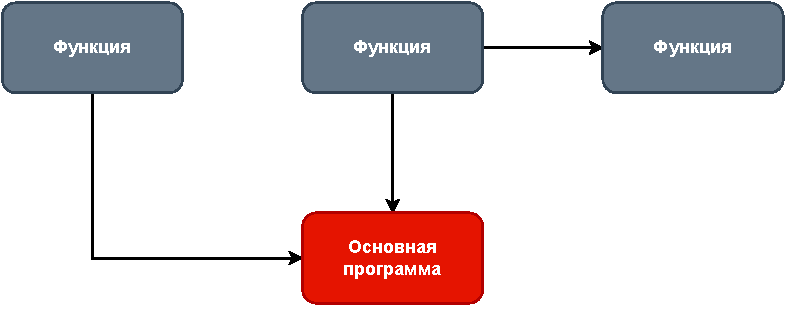
\includegraphics[width=.73\textwidth]{pics/oop1.pdf}
\caption{Схема взаимодействия функций с основной программой и между собой}
\end{figure}
\vfill
\end{frame}


\begin{frame}[fragile]{Зачем использовать ООП}
\scriptsize
\begin{itemize}
\item Существенный недостаток процедурного подхода~-- части кода сильно зависят друг от друга.
\end{itemize}
\begin{minipage}{.35\textwidth}
\begin{itemize}
\item При изменении какой-либо функции, остальные части программы могут быть к этому не готовы~-- программа в целом может сломаться.
\item В процедурном программировании часто приходится писать повторяющийся код и реализовывать похожие функции с небольшими отличиями.
\end{itemize}
\vfill
\end{minipage}
\begin{minipage}{.64\textwidth}
\begin{figure}[h!]
\centering
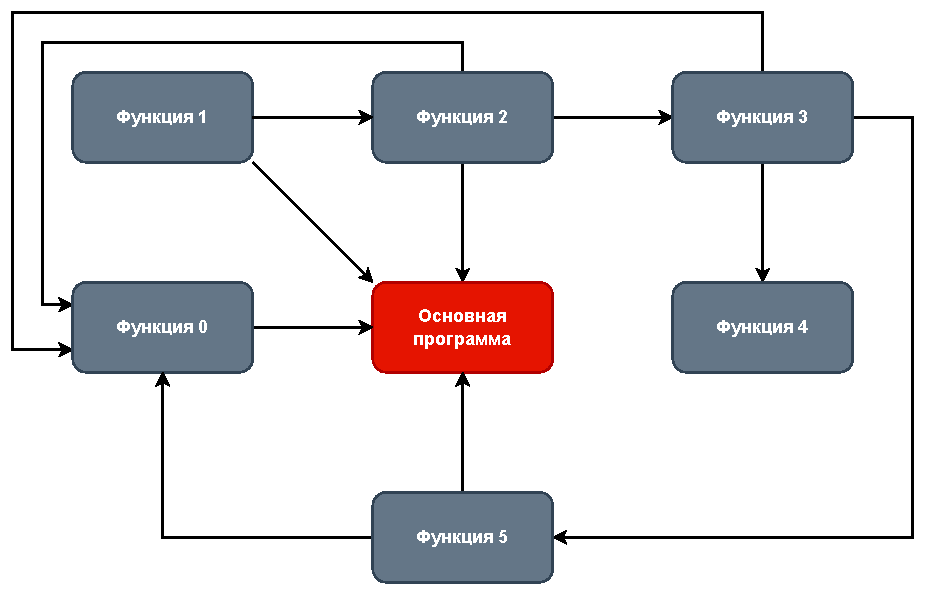
\includegraphics[width=\linewidth]{pics/oop2.pdf}
\caption{Недостатки процедурного подхода}
\end{figure}
\end{minipage}
\vfill
\end{frame}


\begin{frame}[fragile]{Зачем использовать ООП}
\scriptsize
\begin{minipage}{.54\textwidth}
\begin{itemize}
\item Логика ООП абсолютно другая: к основной программе подключаются не функции, а объекты, внутри которых уже есть собственные переменные и функции.
\item Выстраивается более иерархичная структура.
\item Объекты независимы друг от друга и самодостаточны: если сломать что-то в одном объекте, это никак не отразится на работе других.
\item Даже если полностью изменить содержание объекта, но сохранить при этом его поведение, весь код продолжит работать.
\end{itemize}
\end{minipage}
\begin{minipage}{.45\textwidth}
\begin{figure}[h!]
\centering
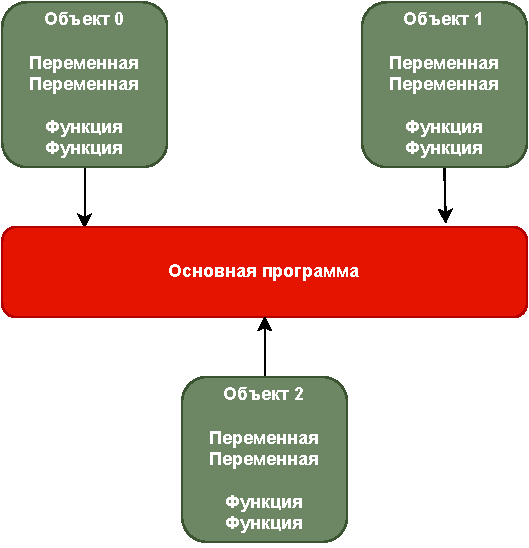
\includegraphics[width=\linewidth]{pics/oop3.pdf}
\caption{Схема ООП}
\end{figure}
\end{minipage}
\vfill
\end{frame}


\subsection{Работа с классами}
\begin{frame}[fragile]{Работа с классами}
\scriptsize
Каждый объект в ООП строится по определенному классу~-- абстрактной модели, описывающей из чего состоит объект и что с ним можно делать.
\vfill
Например, у нас есть класс <<Car>> с полями <<brand>>, <<color>>, <<power>> и методами <<go>> и <<brake>>.

Если присвоить полям определенные значения, можно создать вполне конкретные объекты.
\vfill
Допустим:
\begin{enumerate}
\item \mintinline{python}|brand = 'Porshe'|
\item \mintinline{python}|color = 'white'|
\item \mintinline{python}|power = 353|
\end{enumerate}
\vfill
Таким образом, можно создать сколько угодно различных объектов класса \mintinline{python}|Car|.
\vfill
\begin{figure}[h!]
\centering
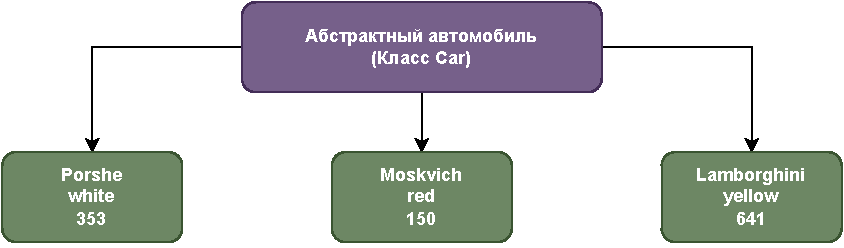
\includegraphics[width=.7\textwidth]{pics/car.pdf}
\caption{Класс <<Car>> и его экземпляры}
\end{figure}
\begin{itemize}
\item При этом для любого объекта класса <<Car>> будут доступны методы <<go>> и <<brake>>.
\end{itemize}
\vfill
\end{frame}


\section{Основные понятия ООП в языке Python}
\sectionframe

\begin{frame}[fragile]{Основные понятия ООП в языке Python}
\scriptsize
Основные понятия объектно-ориентированного программирования: \textcolor{tpugreen}{\textbf{инкапсуляция}}, \textbf{наследование}, \textcolor{tpugreen}{\textbf{полиморфизм}} и \textbf{абстракция}.
Рассмотрим данные понятия на примере класса <<Car>>.
\vfill
\begin{minted}{python}
class Car:
    def __init__(self, brand: str,
                 color: str, power: float) -> None:

        self.brand = brand
        self.color = color
        self.power = power
        self.speed = 0

    def go(self, acceleration_speed: float) -> None:
        self.speed += acceleration_speed

    def brake(self, braking_speed: float) -> None:
        self.speed -= braking_speed
|\space|
\end{minted}
\vfill
\end{frame}


\begin{frame}[fragile]{Основные понятия ООП в языке Python}
\scriptsize
\begin{itemize}
\item Метод \mintinline{python}|__init__()|~-- конструктор (инициализатор) класса. Данный метод вызывается сразу после создания объекта, для того, чтобы присваивать значения динамическим атрибутам.
\item \mintinline{python}|self|~-- ссылка на текущий объект, предоставляющая доступ к полям и методам объекта, с которым Вы работаете.
\item Имена классов принято писать с заглавной буквы, а объектов~-- со строчной.
\end{itemize}
\vfill
Создадим несколько объектов класса <<Car>>:
\vfill
\begin{minted}[firstnumber=last]{python}
car1 = Car(brand='Audi', color='black', power=350)
car2 = Car(brand='BMW', color='special blue', power=375)

print(car1.brand, car1.power, car1.color)
print(car2.brand, car2.power, car2.color)
|\space|
\end{minted}
\begin{minted}{pycon}
Audi 249 black
BMW 375 special blue
\end{minted}
\vfill
\end{frame}

\subsection{Инкапсуляция}
\begin{frame}[fragile]{Инкапсуляция}
\scriptsize
\textcolor{tpugreen}{\textbf{Инкапсуляция}}~-- механизм сокрытия деталей реализации класса от других объектов.
\vfill
Достигается путем использования модификаторов доступа:
\begin{enumerate}
\item \textbf{\texttt{public}}: \mintinline{python}|x|,
\item \textbf{\texttt{private}}: \mintinline{python}|__x|,
\item \textbf{\texttt{protected}}: \mintinline{python}|_x|,
\end{enumerate}
которые соответствуют публичным, приватным и защищенным атрибутам.
\vfill
\begin{itemize}
\item Доступ к данным объекта должен контролироваться, чтобы пользователь не мог изменять их в произвольном порядке и, тем самым, что-то сломать.
\item Для работы с данными лучше написать специальные методы, которые можно будет использовать вне класса, ничего не сломав внутри.
\end{itemize}
\vfill
Разрешим изменять в классе <<\texttt{Car}>> поля <<\texttt{power}>> и <<\texttt{color}>>, а поле <<\texttt{brand}>> сделаем доступным только для чтения, т.к. его изменить нельзя.
\vfill
\end{frame}


\begin{frame}[fragile]{Инкапсуляция}
\scriptsize
\begin{minted}{python}
class Car:
    def __init__(self, brand: str,
                 color: str, power: float) -> None:
        self.__brand = brand  # приватный атрибут (private)
        self.color = color  #  публичный атрибут (public)
        self._power = power  # защищенный атрибут (protected)
        self.__speed = 0  # приватный атрибут (private)

    def go(self, acceleration_speed: float) -> None:
        self.__speed += acceleration_speed

    def brake(self, braking_speed: float) -> None:
        self.__speed -= braking_speed

    def paint(self, color: str) -> None:
        self.color = color
|\space|
\end{minted}
\vfill
\end{frame}


\begin{frame}[fragile]{Инкапсуляция}
\scriptsize
\begin{minted}[firstnumber=last]{python}
    @property
    def brand(self) -> str:
        return self.__brand

    @property
    def power(self) -> float:
        return self._power

    @power.setter
    def power(self, power: float) -> None:
        if power > self._power:
            self._power = power
|\space|
\end{minted}
\begin{itemize}
\item \mintinline{python}|@property|~-- это декоратор\footnote{\tiny{\textcolor{tpugreen}{\textbf{Декораторы}} представляют функцию, которая в качестве параметра получает функцию и в качестве результата также возвращает функцию. Декораторы позволяют модифицировать выполняемую функцию, значения ее параметров и ее результат без изменения исходного кода этой функции.}}, который обрабатывает получение значения переменной класса. Для каждого свойства объявляется свой метод: \mintinline{python}|brand| и \mintinline{python}|power|. В этих методах мы возвращаем значения закрытых атрибутов.
\item \mintinline{python}|@power.setter|~-- декоратор, который определяет, что делать при установке значения переменной \mintinline{python}|power|.
\end{itemize}
\vfill
\end{frame}


\begin{frame}[fragile]{Инкапсуляция}
\scriptsize
Создадим экземпляр класса \mintinline{python}|Car|:
\vfill
\begin{minted}[firstnumber=last]{python}
|\space|
my_car = Car(brand='Audi', color='black', power=249)
print(my_car.power, my_car.brand, my_car.color)

my_car.power = 320
print(my_car.power, my_car.brand, my_car.color)

my_car.paint('white')
print(my_car.power, my_car.brand, my_car.color)
|\space|
\end{minted}
\begin{minted}{pycon}
249 Audi black
320 Audi black
320 Audi white
\end{minted}
\vfill
\end{frame}


\subsection{Наследование}
\begin{frame}[fragile]{Наследование}
\scriptsize
\textcolor{tpugreen}{\textbf{Наследование}}~-- концепция объектно-ориентированного программирования, согласно которой абстрактный тип данных может наследовать данные и функциональность некоторого существующего типа, способствуя повторному использованию компонентов программного обеспечения.
\begin{itemize}
\item Классы могут передавать свои атрибуты и методы классам-потомкам.
\item Новый класс, называемый \textbf{подклассом} или \textbf{производным} классом, наследует свойства и методы существующего класса, называемого \textbf{суперклассом} или \textbf{базовым} классом.
\end{itemize}
\vfill
\begin{minted}{python}
class GasolineCar(Car):
    def __init__(self, brand: str,
                 color: str, power: float, engine: str) -> None:
        super().__init__(brand, color, power)
        self.__engine = engine

    @property
    def engine(self) -> str:
        return self.__engine

    def charge(self, volume: float) -> str:
        return f'Заправить {volume} литров бензина'
|\space|
|\space|
\end{minted}
\vfill
\end{frame}


\begin{frame}[fragile]{Наследование}
\scriptsize
\begin{minted}[firstnumber=last]{python}
class ElectricCar(GasolineCar):
    def charge(self, volume: float) -> str:
        value = super().charge(volume)
        return value.replace('литров бензина', 'ватт электричества')


my_car = GasolineCar(brand='Jaguar', color='red', power=550, engine='gasoline')
print(my_car.charge(50))

my_car2 = ElectricCar(brand='Tesla', color='white', power=1020, engine='electric')
print(my_car2.charge(10_000))
|\space|
\end{minted}
\begin{minted}{pycon}
Заправить 50 литров бензина
Заправить 10000 ватт электричества
\end{minted}
\vfill
\end{frame}


\subsection{Полиморфизм}
\begin{frame}[fragile]{Полиморфизм}
\scriptsize
\textcolor{tpugreen}{\textbf{Полиморфизм}}~-- это принцип, позволяющий применять одни и те же команды к объектам разных классов, даже в том случае, если они выполняются по-разному.
\vfill
\begin{minted}{python}
class Cat:
    def sleep(self) -> None:
        print('Свернулся в клубок и сладко спит')

class Parrot:
    def sleep(self) -> None:
        print('Сел на жёрдочку и уснул')

def home_sleep(somebody: object) -> None:
    somebody.sleep()

cat = Cat()
parrot = Parrot()
home_sleep(cat)
home_sleep(parrot)
|\space|
\end{minted}
\begin{minted}{pycon}
Свернулся в клубок и сладко спит
Сел на жёрдочку и уснул
\end{minted}
\vfill
\end{frame}


\subsection{Абстракция}
\begin{frame}[fragile]{Абстракция}
\scriptsize
\textcolor{tpugreen}{\textbf{Абстракция}} данных означает выделение значимой информации и исключение из рассмотрения незначимой (набор значимых характеристик объекта, доступный остальной программе).
\vfill
При создании класса, его упрощают до тех атрибутов, которые нужны именно в этом коде, без попытки описать его целиком, отбрасывая все второстепенное.
\vfill
\begin{minted}{python}
class Predator:
    def hunt(self) -> None:
        print('...hunting...')


class Cat(Predator):
    def __init__(self, name: str, color: str) -> None:
        super().__init__()
        self.name = name
        self.color = color


cat = Cat(name='Felix', color='ginger')
cat.hunt()

|\space|
\end{minted}
\begin{minted}{pycon}
...hunting...
\end{minted}
\vfill
\end{frame}

\section{Переменные класса и объекта}
\sectionframe

\begin{frame}[fragile]{Переменные класса и объекта}
\scriptsize
\begin{itemize}
	\item Поля можно воспринимать как обычные переменные, заключённые в \textbf{пространствах имён} классов и объектов. Их имена действительны только в контексте (пространстве имен) этих классов или объектов.

	\item \textcolor{extraorange}{\textbf{Переменные класса}} разделяемы~-- доступ к ним могут получать все экземпляры этого класса. Переменная класса существует только одна, поэтому когда любой из объектов изменяет переменную класса, это изменение отразится и во всех остальных экземплярах класса.

	\item \textcolor{extraorange}{\textbf{Переменные объекта}} принадлежат каждому отдельному экземпляру класса. В этом случае у каждого объекта есть своя собственная копия поля, т.е. не разделяемая с другими такими же полями в других экземплярах. Доступ к полям объекта осуществляется через переменную \mintinline{python}|self|.
\end{itemize}
\vfill
\end{frame}

\begin{frame}[fragile]{Переменные класса и объекта}
\scriptsize
\begin{minted}{python}
class Droid:
    population = 0

    def __init__(self, name: str) -> None:
        self.name = name
        print(f'** Инициализация {self.name} **')
        Droid.population += 1

    def say_hi(self) -> None:
        print(f'Приветствую! Мои хозяева называют меня {self.name}.')

    @staticmethod
    def how_many():
        print(f'У нас {Droid.population} дроидов.')
|\space|
|\space|
\end{minted}
\vfill
\begin{itemize}
\item Статические методы не могут изменять ни состояние объекта, ни состояние класса. Они работают как обычные функции, но принадлежат пространству имен класса (каждого его экземпляра).
\item Статические методы помечаются декоратором \mintinline{python}|@staticmethod|.
\end{itemize}
\vfill
\end{frame}


\begin{frame}[fragile]{Переменные класса и объекта}
\scriptsize
\begin{minted}[firstnumber=last]{python}
droid1 = Droid('R2D2')
droid1.say_hi()

Droid.how_many()

droid2 = Droid('C-3PO')
droid2.say_hi()
droid2.how_many()

def how_many(obj):
    print(f'У Вас {obj.population} дроидов.')

how_many(Droid)
|\space|
\end{minted}
\begin{minted}{pycon}
** Инициализация R2D2 **
Приветствую! Мои хозяева называют меня R2D2.
У нас 1 дроидов.
** Инициализация C-3PO **
Приветствую! Мои хозяева называют меня C-3PO.
У нас 2 дроидов.
У Вас 2 дроидов.
\end{minted}
\vfill
\end{frame}

\begin{frame}[fragile]{Переменные класса и объекта}
\scriptsize
\begin{minted}{python}
class Droid:
    population = 0

    def __init__(self, name: str) -> None:
        self.name = name
        print(f'** Инициализация {self.name} **')
        Droid.population += 1

    def say_hi(self) -> None:
        print(f'Приветствую! Мои хозяева называют меня {self.name}.')

    def __len__(self):
        return self.population
|\space|
|\space|
\end{minted}
\vfill
\begin{itemize}
\item Специальный (магический\footnote{\tiny{<<\textbf{Магические методы}>>}~-- это методы, которые позволяют объектам классов взаимодейстовать со встроенными функциями и операторами языка Python.}, dunder\footnote{\tiny{dunder~-- сокращение от <<double underscore>>~-- двойное подчеркивание}}) метод \mintinline{python}|__len__()| позволяет определить поведение экземпляра пользовательского класса при запросе его длины с помощью функции \mintinline{python}|len()|.
\end{itemize}
\vfill
\end{frame}


\begin{frame}[fragile]{Переменные класса и объекта}
\scriptsize
\begin{minted}[firstnumber=last]{python}
droid1 = Droid('R2D2')
droid1.say_hi()
print(f'У Вас {len(droid1)} дроидов')

droid2 = Droid('C-3PO')
droid2.say_hi()
print(f'У Вас {len(droid2)} дроидов')
print(len(droid1) == len(droid2))
|\space|
\end{minted}
\begin{minted}{pycon}
** Инициализация R2D2 **
Приветствую! Мои хозяева называют меня R2D2.
У Вас 1 дроидов
** Инициализация C-3PO **
Приветствую! Мои хозяева называют меня C-3PO.
У Вас 2 дроидов
True
\end{minted}
\vfill
\end{frame}

\section{Реализация ХТС с помощью \\ объектной модели}
\sectionframe

\begin{frame}[fragile]{Реализация ХТС с помощью объектной модели}
\scriptsize
\begin{itemize}
\item Рассмотрим простую химико-технологическую систему, состоящую из 3-х потоков и смесителя.
\end{itemize}
\vfill
\begin{figure}[h!]
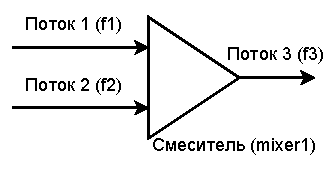
\includegraphics[width=.5\textwidth]{./pics/pfd}
\caption{Блок-схема химико-технологической системы (ХТС)\footnote{\tiny{В скобках указаны имена соответствующих переменных, используемых в программном коде.}}}
\end{figure}
\vfill
\begin{itemize}
\item Реализуем отдельные классы для описания объектов потока и смесителя.
\end{itemize}
\vfill
\end{frame}

\subsection{Описание класса \texttt{Flow}}

%\begin{frame}[fragile]{Описание класса \texttt{Flow}}
%\scriptsize
%\begin{table}[h!]
%	\centering
%	\renewcommand{\arraystretch}{1.2}
%	\begin{tabular}{|p{.49\linewidth}|p{.49\linewidth}|}
%		\hline
%		\textbf{Атрибуты класса} & \textbf{Описание}  \\
%		\hline
%		\mintinline{python}|mass_flow_rate: float| & Массовый расход, кг/ч \\
%		\hline
%		\mintinline{python}|mass_fractions: np.ndarray| & Массовые доли \\
%		\hline
%		\mintinline{python}|temperature: float| & Температура потока, °C \\
%		\hline
%		\mintinline{python}|pressure: float| & Давление потока, кПа \\
%		\hline
%\begin{minipage}{\linewidth}
%\begin{minted}[frame=none, linenos=false]{python}
%def __init__(
%    self,
%    mass_flow_rate: float,
%    mass_fractions: np.ndarray,
%    temperature: float, pressure: float
%) -> None
%\end{minted}
%\end{minipage}
%		& Создает новый экземпляр класса \texttt{Flow}, заполняя все поля \\
%		\hline
%\begin{minipage}{\linewidth}
%\begin{minted}[frame=none, linenos=false]{python}
%def convert_mass_to_volume_fractions(
%    self,
%    densities: np.ndarray
%) -> np.ndarray
%\end{minted}
%\end{minipage}
%		& Перевод массовых долей в объемные \\
%		\hline
%\begin{minipage}{\linewidth}
%\begin{minted}[frame=none, linenos=false]{python}
%def convert_mass_to_mole_fractions(
%    self,
%    mr: np.ndarray
%) -> np.ndarray
%\end{minted}
%\end{minipage}
%		& Перевод массовых долей в мольные \\
%		\hline
%	\end{tabular}
%\end{table}
%\vfill
%\end{frame}
%
%\begin{frame}[fragile]{Описание класса \texttt{Flow}}
%\scriptsize
%\begin{table}[h!]
%	\centering
%	\renewcommand{\arraystretch}{1.2}
%	\begin{tabular}{|p{.49\linewidth}|p{.49\linewidth}|}
%		\hline
%		\textbf{Атрибуты класса} & \textbf{Описание}  \\
%		\hline
%\begin{minipage}{\linewidth}
%\begin{minted}[frame=none, linenos=false]{python}
%def get_flow_density(
%    self,
%    densities: np.ndarray
%) -> float
%\end{minted}
%\end{minipage}
%		& Расчет плотности потока \\
%		\hline
%\begin{minipage}{\linewidth}
%\begin{minted}[frame=none, linenos=false]{python}
%def get_average_molar_mass(
%    self,
%    mr: np.ndarray
%) -> float
%\end{minted}
%\end{minipage}
%		& Расчет средней молекулярной массы потока \\
%		\hline
%	\end{tabular}
%\end{table}
%\vfill
%\end{frame}

%\subsubsection{Функции для пересчета составов}
\begin{frame}[fragile]{Функции для пересчета составов}
\scriptsize
\begin{enumerate}
\item Пересчет массовых долей в объемные:
\vfill
\begin{equation*}
	\varphi _i = \dfrac{\dfrac{\omega _i}{\rho _i}}{\sum \limits _{i=1}^{n} \dfrac{\omega _i}{\rho _i}}
\end{equation*}
\vfill
где $\varphi _i$~-- объемная доля $i$-го компонента; $\omega _i$~-- массовая доля $i$-го компонента; $\rho _i$~-- плотность $i$-го компонента; $n$~-- число компонентов в системе; $i$~-- индекс компонента в системе.
\vfill
\item Пересчет массовых долей в мольные:
\vfill
$$
	\chi _i = \dfrac{\dfrac{\omega _i}{M_i}}{\sum \limits_{i=1}^{n}\dfrac{\omega _i}{M_i}}
$$
\vfill
где $\chi _i$~-- мольная доля $i$-го компонента; $\omega _i$~-- массовая доля $i$-го компонента; $M_i$~-- молярная масса $i$-го компонента; $n$~-- число компонентов в системе; $i$~-- индекс компонента в системе.
\vfill
\end{enumerate}
\vfill
\end{frame}


%\subsubsection{Функции для расчета плотности  и средней \\ молекулярной массы}
\begin{frame}[fragile]{Функции для расчета плотности и средней \\ молекулярной массы}
\scriptsize
\begin{enumerate}
\item Расчет плотности:
\vfill
\begin{equation*}
	\rho = \dfrac{1}{\sum \limits_{i=1}^{n}\dfrac{\omega_i}{\rho_i}}
\end{equation*}
\vfill
где $\rho$~-- плотность потока; $\omega _i$~-- массовая доля $i$-го компонента; $\rho _i$~-- плотность $i$-го компонента; $n$~-- число компонентов в системе; $i$~-- индекс компонента в системе.
\vfill
\item Расчет средней молекулярной массы потока:
\vfill
$$
	m = \dfrac{1}{\sum \limits_{i=1}^{n}\dfrac{\omega_i}{M_i}}
$$
\vfill
где $m$~-- средняя молекулярная масса потока; $\omega _i$~-- массовая доля $i$-го компонента; $M_i$~-- молярная масса $i$-го компонента; $n$~-- число компонентов в системе; $i$~-- индекс компонента в системе.
\vfill
\end{enumerate}
\vfill
\end{frame}

\begin{frame}[fragile]{Модуль вспомогательных функций}
\scriptsize
Файл \texttt{converters\_and\_functions.py}:
\vfill
\begin{minted}{python}
import numpy as np


def convert_mass_to_volume_fractions(
    mass_fractions: np.ndarray,
    density: np.ndarray
) -> np.ndarray:
    x = mass_fractions / density
    s = x.sum()
    return x / s


def convert_mass_to_mole_fractions(
    mass_fractions: np.ndarray,
    mr: np.ndarray
) -> np.ndarray:
    x = mass_fractions / mr
    s = x.sum()
    return x / s
\end{minted}
\vfill
\end{frame}

\begin{frame}[fragile]{Модуль вспомогательных функций}
\scriptsize
\begin{minted}[firstnumber=last]{python}
|\space|
|\space|
def get_flow_density(
    mass_fractions: np.ndarray,
    density: np.ndarray
) -> float:
    return (mass_fractions / density).sum() ** -1


def get_average_mol_mass(
    mass_fractions: np.ndarray,
    mr: np.ndarray
) -> float:
    return (mass_fractions / mr).sum() ** -1
|\space|
|\space|
\end{minted}
\vfill
\end{frame}

\begin{frame}[fragile]{Модуль вспомогательных функций}
\scriptsize
\begin{minted}[firstnumber=last]{python}
def get_flow_cp(
    mass_fractions: np.ndarray,
    coeffs: np.ndarray,
    temperature: float
) -> float:
    p = np.arange(coeffs.shape[1])
    component_cp = ((p + 1) * coeffs * temperature ** p).sum(axis=1)
    return (component_cp * mass_fractions).sum()


def normalize(x: np.ndarray) -> np.ndarray:
    return x / x.sum()
|\space|
|\space|
\end{minted}
\vfill
\end{frame}

%\subsubsection{Программная реализация}
\begin{frame}[fragile]{Программная реализация класса \texttt{Flow}}
\scriptsize
Рассмотрим пример реализации класса \mintinline{python}|Flow|, являющегося представлением объекта материального потока (модуль \texttt{flow.py}). Свойства веществ сохраним в файле \texttt{constants.py}
\vfill
\begin{minted}{python}
import numpy as np
import constants as const
import converters_and_functions as conv


class Flow:
    def __init__(
            self,
            mass_flow_rate: float,
            mass_fractions: np.ndarray,
            temperature: float
    ) -> None:
        self.mass_flow_rate = mass_flow_rate
        self.mass_fractions = mass_fractions
        self.temperature = temperature
        self.mole_fractions = conv.convert_mass_to_mole_fractions(
            self.mass_fractions, const.MR
        )
|\space|
\end{minted}
\vfill
\end{frame}

\begin{frame}[fragile]{Программная реализация класса \texttt{Flow}}
\scriptsize
\begin{minted}[firstnumber=last]{python}
        self.volume_fractions = conv.convert_mass_to_volume_fractions(
            self.mass_fractions, const.DENSITIES
        )
        self.density = conv.get_flow_density(
            self.mass_fractions, const.DENSITIES
        )
        self.average_mol_mass = conv.get_average_mol_mass(
            self.mass_fractions, const.MR
        )
        self.mole_flow_rate = self.mass_flow_rate / self.average_mol_mass
        self.volume_flow_rate = self.mass_flow_rate / (self.density * 1e3)

   @property
   def flow_cp(self) -> float:
       flow_cp = conv.get_flow_cp(
           self.mass_fractions, const.HEATCAPACITYCOEFFS, self.temperature
       )
       return flow_cp
|\space|
|\space|
\end{minted}
\vfill
\end{frame}

\begin{frame}[fragile]{Программная реализация класса \texttt{Flow}}
\scriptsize
\begin{minted}[firstnumber=last]{python}
if __name__ == '__main__':
    x = np.random.randint(1, 5, 24)
    x = conv.normalize(x)
    t = 500
    g = 1000
    f = Flow(mass_flow_rate=g, mass_fractions=x, temperature=t)
    print(f.volume_fractions)
    print(f.density)
    print(f.average_mol_mass)
    print(f.flow_cp)
|\space|
\end{minted}
\begin{minted}{pycon}
[5.37441087e-05 5.15298514e-01 1.04442992e-04 3.19180085e-03
 2.67455976e-05 2.67455976e-05 4.32611950e-05 4.78605431e-01
 7.90739408e-05 8.09030533e-05 7.26318146e-05 5.70721958e-05
 4.70191478e-05 1.62992735e-03 9.26112964e-05 3.49750123e-05
 5.59026836e-05 8.31976504e-05 5.22015109e-05 5.45610192e-05
 3.78895966e-05 8.52515924e-05 9.75232707e-05 8.85730830e-05]
0.001479118741981714
40.69750532482536
2.1877717798631178
    \end{minted}
\vfill
\end{frame}

\subsection{Описание класса \texttt{Mixer}}
\begin{frame}[fragile]{Описание класса \texttt{Mixer}}
\scriptsize
\begin{table}[h!]
	\centering
	\renewcommand{\arraystretch}{1.2}
	\begin{tabular}{|p{.49\linewidth}|p{.49\linewidth}|}
		\hline
		\textbf{Атрибуты класса} & \textbf{Описание}  \\
		\hline
\begin{minipage}{\linewidth}
\vfill
\begin{minted}[frame=none, linenos=false]{python}
def mix(self, *flows: Flow) -> Flow
\end{minted}
\vfill
\end{minipage}
		& Реализация метода смешения потоков. Возвращает результирующий поток в виде объекта класса \texttt{Flow}\\
		\hline
	\end{tabular}
\end{table}
\vfill
Состав смесевого потока (в массовых долях) можно найти следующим образом:
\vfill
$$
	\omega _i = \dfrac{\sum \limits_ {j=1} ^{n} G_j \cdot \omega _{i,j}}{\sum \limits_ {j=1} ^{n} G_j}
$$
\vfill
где $\omega _i$~-- массовая доля $i$-го компонента; $G_j$~-- массовый расход $j$-го потока, кг/ч; $\omega _{i,j}$~-- массовая доля $i$-го компонента в $j$-ом потоке; $n$~-- количество смешиваемых потоков.
\vfill
\vfill
\end{frame}

%\subsubsection{Программная реализация}
\begin{frame}[fragile]{Программная реализация класса \texttt{Mixer}}
\scriptsize
Файл \texttt{mixer.py}:
\begin{minted}{python}
import numpy as np
from scipy.optimize import fsolve
from flows import Flow


class Mixer:
    def mix(self, *flows: Flow) -> Flow:
        self.flows = flows
        mass_flow_rate = np.sum(
            [flow.mass_flow_rate for flow in self.flows]
        )
        mass_fractions = np.sum(
            [flow.mass_fractions * flow.mass_flow_rate for flow in self.flows],
            axis=0,
        ) / mass_flow_rate
        t_mean = np.mean(
            [flow.temperature for flow in self.flows]
        )
|\space|
\end{minted}
\vfill
\end{frame}

\begin{frame}[fragile]{Программная реализация класса \texttt{Mixer}}
\scriptsize
\begin{minted}[firstnumber=last]{python}
        self.mixture = Flow(
            mass_flow_rate=mass_flow_rate,
            mass_fractions=mass_fractions,
            temperature=t_mean
        )
        self.mixture.temperature = self.__calculate_temperature()
        return self.mixture

    def __calculate_temperature(self) -> float:
        def func(t):
            self.mixture.temperature = t
            t_ = np.sum(
                [flow.mass_flow_rate * flow.flow_cp * flow.temperature
                 for flow in self.flows]
            ) / (self.mixture.mass_flow_rate * self.mixture.flow_cp)
            return t - t_

        temperature, = fsolve(func, self.mixture.temperature)
        return temperature
|\space|
|\space|
\end{minted}
\vfill
\end{frame}

\begin{frame}[fragile]{Программная реализация класса \texttt{Mixer}}
\scriptsize
\begin{minted}[firstnumber=last]{python}
if __name__ == '__main__':
    import converters_and_functions as conv

    f1 = Flow(
        mass_flow_rate=100,
        mass_fractions=conv.normalize(np.random.randint(1, 5, 24)),
        temperature=200
    )
    f2 = Flow(
        mass_flow_rate=100,
        mass_fractions=conv.normalize(np.random.randint(1, 5, 24)),
        temperature=300
    )
    m = Mixer()
    fmixture = m.mix(f1, f2)
    print(fmixture.temperature)
|\space|
\end{minted}
\begin{minted}{pycon}
249.13760300860477
\end{minted}
\vfill
\end{frame}


\subsection{Описание основной программы}
\begin{frame}[fragile]{Описание основной программы}
\scriptsize
\begin{minted}{python}
import numpy as np
from flow import Flow
from mixer import Mixer
import constants as const


if __name__ == '__main__':
    mf1 = np.array(
        [
            .1, .1, .1, .4, .2, .05, .03, .02,
            .0, .0, .0, .0, .0, .0,  .0,  .0,
            .0, .0, .0, .0, .0, .0,  .0,  .0,
        ]
    )
    mf2 = np.array(
        [
            .0, .0, .2, .5, .1, .15, .0, .05,
            .0, .0, .0, .0, .0, .0,  .0, .0,
            .0, .0, .0, .0, .0, .0,  .0, .0,
        ]
    )
\end{minted}
\vfill
\end{frame}


\begin{frame}[fragile]{Описание основной программы}
\scriptsize
\begin{minted}[firstnumber=last]{python}
    f1 = Flow(
        mass_flow_rate=100,
        mass_fractions=mf1,
        temperature=130
    )
    f2 = Flow(
        mass_flow_rate=120,
        mass_fractions=mf2,
        temperature=120
    )
    mixer1 = Mixer()
    f3 = mixer1.mix(f1, f2)
    print(f3.mass_flow_rate, f3.temperature)
    print(f3.mass_fractions)
\end{minted}
\vfill
\begin{minted}{pycon}
220 126.42767662034315
[0.04545455 0.04545455 0.15454545 0.45454545 0.14545455 0.10454545
 0.01363636 0.03636364 0.         0.         0.         0.
 0.         0.         0.         0.         0.         0.
 0.         0.         0.         0.         0.         0.        ]
\end{minted}
\vfill
\end{frame}


\contactsframe[\Large \textbf{Благодарю за внимание!}]{

\bigskip

\includegraphics[width=.05\textwidth]{pics/home} \quad Учебный корпус №2, ауд. 136 \\

\includegraphics[width=.05\textwidth]{pics/mail} \quad chuva@tpu.ru \\

\includegraphics[width=.03\textwidth]{pics/tel} \quad +7-962-782-66-15
}

\end{document}

